\documentclass[11pt,a4paper]{article}

% ---------- Packages ----------
\usepackage[utf8]{inputenc}
\usepackage[T1]{fontenc}
\usepackage{lmodern}
\usepackage{amsmath,amssymb}
\usepackage{enumitem}
\usepackage{geometry}
\usepackage{fancyhdr}
\usepackage[most]{tcolorbox}   % enhanced, breakable
\usepackage{hyperref}

% ---------- Geometry ----------
\geometry{margin=2.5cm}

% ---------- Header/Footer ----------
\setlength{\headheight}{14pt}  % fancyhdr warning verhindern
\pagestyle{fancy}
\fancyhf{}
\lhead{Einführung in die Elektrotechnik}
\rhead{Wintersemester 2025}
\cfoot{\thepage}

% ---------- Exercise Environment ----------
\newcounter{exercise}
\newenvironment{exercise}[1][]
  {\refstepcounter{exercise}%
   \begin{tcolorbox}[enhanced, breakable, width=\textwidth,
     colback=blue!5!white,colframe=blue!60!black,
     fonttitle=\bfseries\large,
     title=Aufgabe~\theexercise:~#1]}
  {\end{tcolorbox}}

% ---------- Solution Environment ----------
\newif\ifshowsolutions
\showsolutionstrue  % comment to hide solutions

\newenvironment{solution}
  {\ifshowsolutions
     \begin{tcolorbox}[enhanced, breakable, width=\textwidth,
       colback=green!5!white,colframe=green!50!black,
       fonttitle=\bfseries\large,
       title=Lösung]}
  {\end{tcolorbox}\fi}

% ---------- Document ----------
\begin{document}

% ----- Header Box -----
\begin{tcolorbox}[enhanced, breakable, colback=gray!10!white,
  colframe=gray!70!black, fonttitle=\bfseries\large,
  title={Aufgabenblatt \#4}: Elektrisches Feld]
\begin{center}
  Besprechung: 12.11.2025\end{center}
\end{tcolorbox}
\vspace{1cm}

% ----- Exercise 1 -----
\begin{exercise}[Diskrete Ladungsverteilung]
Zwei Punktladungen von jeweils $+3.0\, \mu\mathrm{C}$ befinden sich an den Punkten $(x, y) = (0, 2.0\, \mathrm{m})$ und $(x, y) = (0, -2.0\, \mathrm{m})$. Zwei weitere Punktladungen, jeweils mit Ladung $q$, befinden sich an den Punkten $(x, y) = (4.0\, \mathrm{m}, 2.0\, \mathrm{m})$ und $(x, y) = (4.0\, \mathrm{m}, -2.0\, \mathrm{m})$. Das elektrische Feld am Punkt $(x, y) = (0, 0)$ aufgrund der vier Ladungen beträgt $\vec{E} = (4.0 \times 10^{3}~\hat{x})~\mathrm{N/C}$. Bestimmen Sie den Wert von $q$.
\end{exercise}

\ifshowsolutions
\begin{solution}
Das elektrische Feld am Ursprung aufgrund einer Punktladung $Q$ an der Position $(x, y)$ ist gegeben durch
\[
\vec{E} = \frac{1}{4\pi \varepsilon_0} \frac{Q}{r^2} \, \hat{r},
\]
wobei $\hat{r}$ der Einheitsvektor ist, der von der Ladung zum Feldpunkt zeigt.

Für die beiden Ladungen bei $(0, 2\, \mathrm{m})$ und $(0, -2\, \mathrm{m})$ zeigen die elektrischen Feldkomponenten am Ursprung entlang der $y$-Achse. Da sie gleich groß und entgegengesetzt gerichtet sind, heben sie sich gegenseitig auf:
\[
E_y = 0 \quad \text{(net field from the two $3.0\, \mu\mathrm{C}$ charges)}
\]

Der Abstand jeder $q$-Ladung zum Ursprung ist
\[
r = \sqrt{(4.0)^2 + (2.0)^2}\, \mathrm{m} = \sqrt{20}\, \mathrm{m},
\]
und das elektrische Feld am Ursprung aufgrund einer der $q$-Ladungen hat die Größe
\[
E_q = \frac{1}{4\pi\varepsilon_0} \frac{|q|}{r^2}.
\]

Am Ursprung heben sich die $y$-Komponenten der Felder der Ladungen bei $(4\, \mathrm{m}, 2\, \mathrm{m})$ und $(4\, \mathrm{m}, -2\, \mathrm{m})$ auf, während die $x$-Komponenten sich addieren.

Demnach beträgt die Gesamtfeldstärke am Ursprung aufgrund beider $q$-Ladungen
\[
|E_x| = 2 \cdot E_q \cos\theta,
\]
wobei $\cos\theta = \frac{x}{r} = \frac{4}{4.472} = 0.894$.

Mit dem Gesamtfeld am Ursprung von
\[
E_x = 4.0 \times 10^3\, \mathrm{N/C},
\]
ergibt sich
\[
q = -\frac{E_x \cdot 4\pi\varepsilon_0 \cdot r^2}{2 \cdot \cos\theta} = -\frac{4.0 \times 10^3 \cdot 2\pi \cdot 8.854 \times 10^{-12} \cdot 20}{0.894}\, \mathrm{C} = -5.0\, \mu\mathrm{C}.
\]
\end{solution}
\fi

% ----- Exercise 2 -----
\begin{exercise}[Gaußsches Gesetz]
Eine massive, nicht leitende Kugel mit Radius \(R\) trägt eine Gesamtladung \(Q\), die gleichmäßig über ihr Volumen verteilt ist. Mithilfe des Gaußschen Gesetzes soll die Größe des elektrischen Feldes \(E(r)\) als Funktion des radialen Abstands \(r\) vom Zentrum bestimmt werden für:
\begin{enumerate}[label=\alph*)]
  \item \(0 \le r < R\) (innerhalb der Kugel),
  \item \(r \ge R\) (außerhalb der Kugel).
\end{enumerate}
Die Ausdrücke sind in Abhängigkeit von \(Q\), \(R\), \(r\) und der Permittivität des freien Raums \(\varepsilon_0\) anzugeben.
\end{exercise}

\ifshowsolutions
\begin{solution}
Da die Ladung gleichmäßig über eine Kugel verteilt ist, ist das Problem kugelsymmetrisch. Das elektrische Feld muss daher radial sein und an jedem Punkt auf einer kugelförmigen Oberfläche, die mit der geladenen Kugel konzentrisch ist, die gleiche Größe haben. Wir wählen eine kugelförmige Gaußsche Oberfläche mit Radius \(r\), die mit der geladenen Kugel konzentrisch ist.

Das Gaußsche Gesetz lautet:
\[
\oint_{\mathcal{S}} \mathbf{E}\cdot d\mathbf{A}=\frac{Q_{\mathrm{enc}}}{\varepsilon_0}.
\]
Auf der gewählten kugelförmigen Oberfläche ist das Feld radial und betragsmäßig konstant, und \(d\mathbf{A}\) ist radial, sodass
\[
\oint_{\mathcal{S}} \mathbf{E}\cdot d\mathbf{A}=E(r)\cdot 4\pi r^2.
\]

Wir berechnen nun \(Q_{\mathrm{enc}}\) für die beiden Bereiche.

\begin{enumerate}[label=\alph*)]
\item Außerhalb der Kugel: \(r\ge R\)

Für \(r\ge R\) umschließt die Gaußsche Oberfläche die gesamte Ladung \(Q\). Somit ist \(Q_{\mathrm{enc}}=Q\), und das Gaußsche Gesetz ergibt:
\[
E(r)\,4\pi r^2=\frac{Q}{\varepsilon_0}
\quad\Rightarrow\quad
E(r)=\frac{Q}{4\pi\varepsilon_0\,r^2},\qquad r\ge R.
\]
Dies ist identisch mit dem elektrischen Feld einer Punktladung \(Q\), die sich im Zentrum befindet.

\item Innerhalb der Kugel: \(0\le r< R\)
Zunächst berechnen wir die Volumenladungsdichte \(\rho\). Das Gesamtvolumen der Kugel ist \(\tfrac{4}{3}\pi R^3\), also
\[
\rho=\frac{Q}{\tfrac{4}{3}\pi R^3}=\frac{3Q}{4\pi R^3}.
\]
The charge enclosed by a Gaussian sphere of radius \(r<R\) is the charge occupying a smaller sphere of radius \(r\):
Die von einer Gaußschen Kugel mit Radius \(r<R\) eingeschlossene Ladung ist diejenige, die in einer kleineren Kugel mit Radius \(r\) enthalten ist:
\[
Q_{\mathrm{enc}}=\rho\cdot \frac{4}{3}\pi r^3
= \frac{3Q}{4\pi R^3}\cdot \frac{4}{3}\pi r^3
= Q\frac{r^3}{R^3}.
\]
Anwendung des Gaußschen Gesetzes:
\[
E(r)\,4\pi r^2=\frac{Q_{\mathrm{enc}}}{\varepsilon_0}
=\frac{Q}{\varepsilon_0}\frac{r^3}{R^3}.
\]
Lösen nach \(E(r)\):
\[
E(r)=\frac{Q}{4\pi\varepsilon_0}\cdot\frac{r}{R^3},\qquad 0\le r< R.
\]
Demnach nimmt die Feldstärke innerhalb der Kugel linear mit \(r\) zu.
\end{enumerate}

Kombiniertes (stückweises) Ergebnis:
\[
E(r)=
\begin{cases}
\dfrac{Q}{4\pi\varepsilon_0}\dfrac{r}{R^3}, & 0\le r< R,\\[8pt]
\dfrac{Q}{4\pi\varepsilon_0\,r^2}, & r\ge R.
\end{cases}
\]
Die Richtung ist radial nach außen, wenn \(Q>0\) ist, und radial nach innen, wenn \(Q<0\) ist.

\bigskip

\textbf{Anmerkungen:}\begin{itemize}
  \item Kontinuität an der Oberfläche: Bei \(r=R\) ergibt der innere Ausdruck \(Q/(4\pi\varepsilon_0 R^2)\), was mit dem äußeren Ausdruck bei \(r=R\) übereinstimmt. Das Feld ist also an der Oberfläche stetig.
  \item Im Zentrum \(r=0\) ist \(E(0)=0\) (aus der inneren Formel), was mit der Symmetrie übereinstimmt.
  \item Außerhalb der Kugel ist das Feld identisch mit dem einer Punktladung \(Q\) im Zentrum.
\end{itemize}
\end{solution}
\fi

% ----- Exercise 3 -----
\begin{exercise}[Kondensatoren im Gleichstrombetrieb]
Bestimme die Spannungen über den Kondensatoren im untenstehenden Schaltbild im stationären Gleichstrombetrieb.

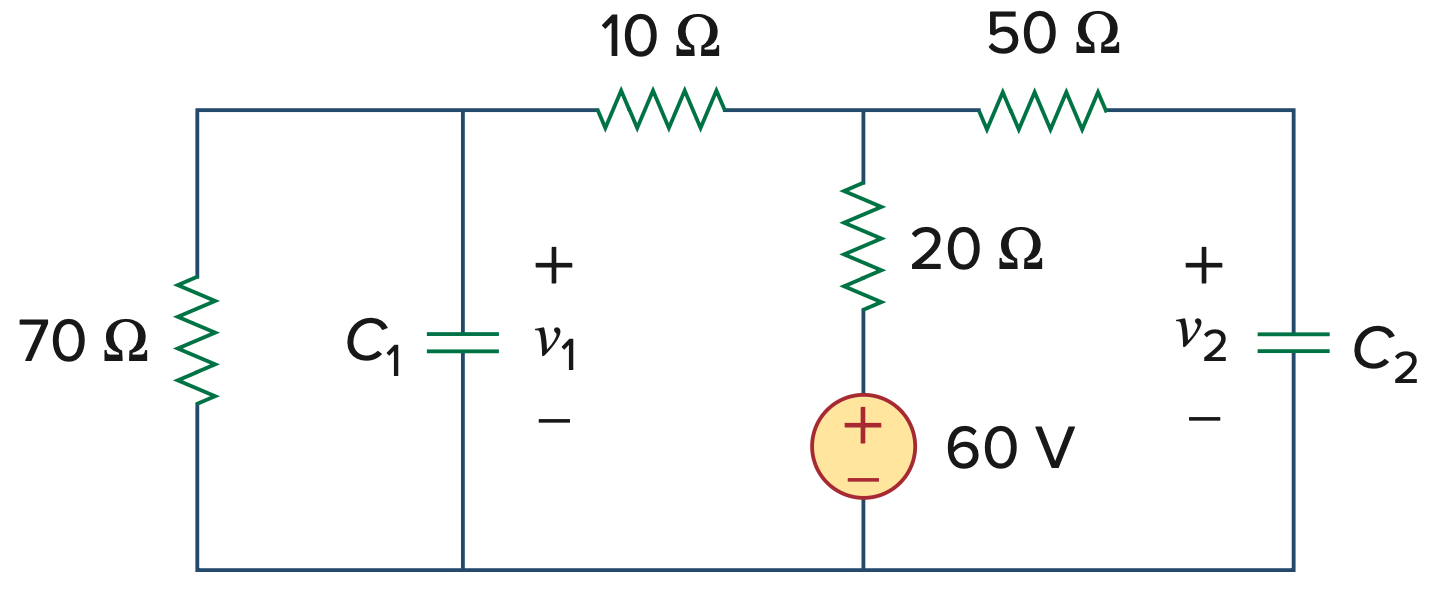
\includegraphics[width=0.7\textwidth]{figures/capacitors.png}
\end{exercise}

\ifshowsolutions
\begin{solution}
Im stationären Gleichstrombetrieb verhalten sich die Kondensatoren wie offene Schaltkreise.
Daher fließt kein Strom durch \( C_1 \) oder \( C_2 \), und wir können einfach das Widerstandsnetzwerk analysieren.

Der untere Knoten sei die Referenz (0 V).
Die Spannung an der Oberseite der \( 60\text{ V} \)-Quelle ist \( V_C = 60\text{ V} \).
\( V_A \) und \( V_B \) seien die Knotenpotentiale an der Oberseite von \( C_1 \) bzw. am Knoten zwischen den \( 10\:\Omega \)-, \( 20\:\Omega \)- und \( 50\:\Omega \)-Widerständen.

\[
\text{KCL am Knoten } A: \quad \frac{V_A - 0}{70} + \frac{V_A - V_B}{10} + I_{C_1} = 0
\]
\[
\Rightarrow \frac{V_A - 0}{70} + \frac{V_A - V_B}{10} = 0
\]

\[
\text{KCL am Knoten } B: \quad \frac{V_B - V_A}{10} + \frac{V_B - 60}{20} + I_{C_2} = 0
\]
\[
\Rightarrow \frac{V_B - V_A}{10} + \frac{V_B - 60}{20} = 0
\]

Multipliziere die erste Gleichung mit \(70\):
\[
V_A + 7(V_A - V_B) = 0 \quad \Longrightarrow \quad 8V_A - 7V_B = 0
\]

Multipliziere die zweite Gleichung mit \(20\):
\[
2(V_B - V_A) + (V_B - 60) = 0 \quad \Longrightarrow \quad -2V_A + 3V_B = 60
\]

Einsetzen ineinander:
\[
-2\left(\frac{7}{8}V_B\right) + 3V_B = 60
\]

\[
\Rightarrow \left(-\frac{14}{8} + \frac{24}{8}\right)V_B = 60
\]

\[
\Rightarrow V_B = 60 \cdot \frac{8}{10} = 48~\text{V}
\]

\[
V_A = \frac{7}{8}V_B = \frac{7}{8} \cdot 48 = 42~\text{V} = v_1
\]

Schließlich sei \( V_D \) die triviale Knotenspannung (nur ein Eingang und ein Ausgang) zwischen der Oberseite von \( C_2 \) und dem \( 50\:\Omega \)-Widerstand.
\[
\text{KCL am Knoten } D: \quad \frac{V_D - V_B}{50} + I_{C_2} = 0 
\]
\[
I_{C_2} = 0 \; (\text{Gleichstrombetrieb}) 
\;\Rightarrow\; \frac{V_D - V_B}{50} = 0 
\;\Rightarrow\; V_D = V_B
\;\Rightarrow\; v_2 = V_B
\]

\[
\boxed{v_1 = 42~\text{V}, \quad v_2 = 48~\text{V}}
\]
\end{solution}
\fi

% ----- Exercise 4 -----
\begin{exercise}[Plattenkondensator]
Wir möchten einen Kondensator mit der Kapazität $C=1\,\mu\mathrm{F}$ entwerfen. Berechne die erforderliche Länge für rechteckige Platten mit einer Breite von $2\,\mathrm{cm}$, wenn das Dielektrikum Polyester ($\varepsilon_r = 3.4$) mit einer Dicke von $15\,\mu\mathrm{m}$ ist.
\end{exercise}

\ifshowsolutions
\begin{solution}
Für einen Plattenkondensator gilt
\[
C = \varepsilon_0 \varepsilon_r \frac{A}{d},
\]
wobei \(A\) die Plattenfläche und \(\varepsilon_0 = 8.85\times 10^{-12}\,\mathrm{F/m}\) die Vakuumpermittivität ist. Für rechteckige Platten gilt \(A = wL\). Lösen nach \(L\) ergibt
\[
L = \frac{C\,d}{\varepsilon_0 \varepsilon_r w} = \frac{1\times 10^{-6} \cdot 15\times 10^{-6}}{8.85\times 10^{-12} \cdot 3.4 \cdot 0.02}\,\mathrm{m} = 24.93\,\mathrm{m}.
\]

Anmerkungen: Diese große Länge ist eine Folge der relativ kleinen Plattenbreite und der bescheidenen relativen Permittivität; um $1\,\mu\mathrm{F}$ mit einer einfachen Plattengeometrie und einem dünnen Polyesterdielektrikum zu erreichen, ist eine sehr große Plattenfläche erforderlich. Praktische Kondensatoren erzielen große Kapazitäten durch die Verwendung mehrerer Schichten, aufgerollter Folien, Dielektrika mit viel höherer Permittivität oder viel kleinerer effektiver Abstände (Dünnfilme, elektrolytische Konstruktionen usw.).
\end{solution}
\fi

% ----- Exercise 5 -----
\begin{exercise}[Zeitabhängige Kondensatorspannungen und -ströme]
Falls $v(0) = 0$ ist, bestimme $v(t)$, $i_1(t)$ und $i_2(t)$ im untenstehenden Schaltbild.

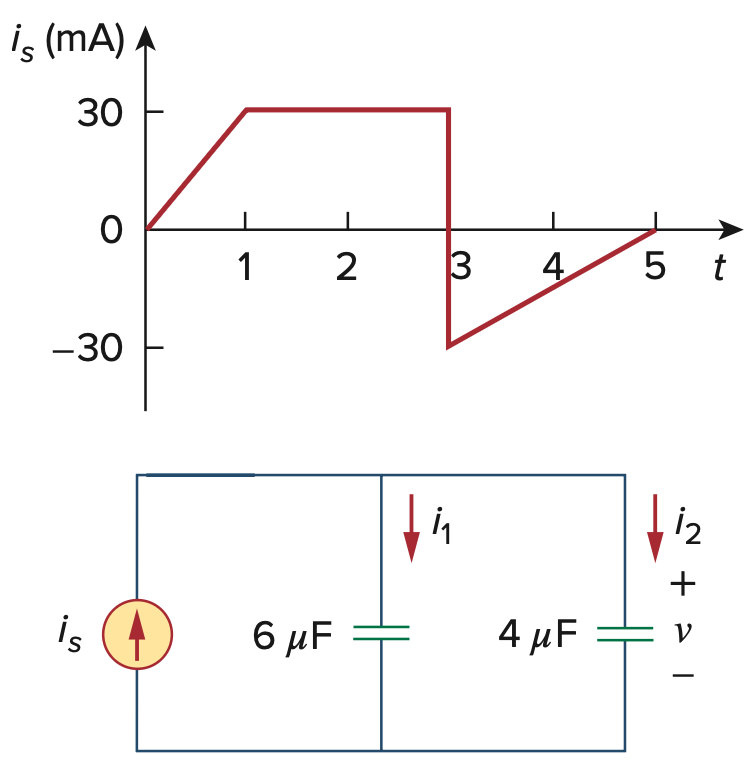
\includegraphics[width=0.7\textwidth]{figures/capacitor_VI.png}
\end{exercise}

\ifshowsolutions
\begin{solution}
\[
i = C \frac{dv}{dt} \Rightarrow v = \frac{\int i\ dt}{C}
\]
Hier gilt,
\[
v(t) = \frac{\int i_s\ dt}{C_{eq}},
\]
mit der äquivalenten Kapazität
\[
C_{eq} = 6\,\mu\mathrm{F} + 4\,\mu\mathrm{F} = 10\,\mu\mathrm{F}.
\]
Für $0 < t < 1\,\mathrm{s}$:
\[
v(t) = \frac{\int 30 t\ dt\,\mathrm{mA} \cdot \mathrm{s}}{10\,\mu\mathrm{F}} = \frac{15 t^2 + \text{const}}{10}\,\mathrm{kV}
\]
\[
v(0) = 0
\]
\[
\Rightarrow \text{const} = 0
\]
\[
\Rightarrow v(t) = 1.5 t^2\,\mathrm{kV}
\]
Für $1 < t < 3\,\mathrm{s}$:
\[
v(t) = \frac{\int 30\ dt}{10}\,\mathrm{kV} = \frac{30 t + \text{const}}{10}\,\mathrm{kV}
\]
\[
v(1\,\mathrm{s}) = 1.5 \cdot 1^2\,\mathrm{kV} = 1.5\,\mathrm{kV}
\]
\[
\Rightarrow \text{const} = 1.5 \cdot 10 - 30 \cdot 1 = -15
\]
\[
\Rightarrow v(t) = (3 t - 1.5)\,\mathrm{kV}
\]
Für $3 < t < 5\,\mathrm{s}$:
\[
v(t) = \frac{\int (\frac{30}{2} t - 75)\ dt}{10}\,\mathrm{kV} = \frac{7.5 t^2 - 75 t  + \text{const}}{10}\,\mathrm{kV}
\]
\[
v(3\,\mathrm{s}) = [1.5 t^2]_0^1\,\mathrm{kV} + [3 t - 1.5]_1^3\,\mathrm{kV} = (1.5 - 0)\,\mathrm{kV} + (7.5 - 1.5)\,\mathrm{kV} = 7.5\,\mathrm{kV}
\]
\[
\Rightarrow \text{const} = 7.5 \cdot 10 - 7.5 \cdot 9 + 75 \cdot 3 = 232.5
\]
\[
\Rightarrow v(t) = (0.75 t^2 - 7.5 t + 23.25)\,\mathrm{kV}
\]
Die Ströme durch jeden Kondensator sind:
\[
i_1 = C_1 \frac{dv}{dt}; \qquad i_2 = C_2 \frac{dv}{dt}
\]
Für $0 < t < 1\,\mathrm{s}$:
\[
i_1 = 6\,\mu\mathrm{F} \cdot 3 t\,\mathrm{kV/s} = 18 t\,\mathrm{mA}
\]
\[
i_2 = 4\,\mu\mathrm{F} \cdot 3 t\,\mathrm{kV/s} = 12 t\,\mathrm{mA}
\]
Für $1 < t < 3\,\mathrm{s}$:
\[
i_1 = 6\,\mu\mathrm{F} \cdot 3\,\mathrm{kV/s} = 18\,\mathrm{mA}
\]
\[
i_2 = 4\,\mu\mathrm{F} \cdot 3\,\mathrm{kV/s} = 12\,\mathrm{mA}
\]
Für $3 < t < 5\,\mathrm{s}$:
\[
i_1 = 6\,\mu\mathrm{F} \cdot (1.5 t - 7.5)\,\mathrm{kV/s} = (9 t - 45)\,\mathrm{mA}
\]
\[
i_2 = 4\,\mu\mathrm{F} \cdot (1.5 t - 7.5)\,\mathrm{kV/s} = (6 t - 30)\,\mathrm{mA}
\]
\end{solution}
\fi

% ----- Exercise 6 -----
\begin{exercise}[Energie von Kondensatoren]
Zwei Kondensatoren ($25\,\mu\mathrm{F}$ und $75\,\mu\mathrm{F}$) sind an eine $100\,\mathrm{V}$-Quelle angeschlossen. Bestimme die in jedem Kondensator gespeicherte Energie, wenn sie folgendermaßen verbunden sind:
\begin{enumerate}[label=\alph*)]
    \item parallel
    \item seriell
\end{enumerate}
\end{exercise}

\ifshowsolutions
\begin{solution}
\begin{enumerate}[label=\alph*)]
\item Die äquivalente Kapazität für Parallelschaltung ist
\[
C_{eq} = C_1 + C_2 = 25\,\mu\mathrm{F} + 75\,\mu\mathrm{F} = 100\,\mu\mathrm{F}.
\]
Die in jedem Kondensator gespeicherte Energie ist
\[
E_1 = \frac{1}{2} \cdot C_1 \cdot V^2 = \frac{1}{2} \cdot 25 \times 10^{-6}\,\mathrm{F} \cdot (100\,\mathrm{V})^2 = 125\,\mathrm{mJ},
\]
\[
E_2 = \frac{1}{2} \cdot C_2 \cdot V^2 = \frac{1}{2} \cdot 75 \times 10^{-6}\,\mathrm{F} \cdot (100\,\mathrm{V})^2 = 375\,\mathrm{mJ}.
\]
\item Die äquivalente Kapazität für Serienschaltung ist
\[
C_{eq} = \frac{C_1 \cdot C_2}{C_1 + C_2} = \frac{25\,\mu\mathrm{F} \cdot 75\,\mu\mathrm{F}}{25\,\mu\mathrm{F} + 75\,\mu\mathrm{F}} = 18.75\,\mu\mathrm{F}.
\]
Die Spannung über jedem Kondensator ist
\[
V_1 = \frac{Q}{C_1} = \frac{C_{eq} \cdot V}{C_1} = \frac{18.75\,\mu\mathrm{F} \cdot 100\,\mathrm{V}}{25\,\mu\mathrm{F}} = 75\,\mathrm{V},
\]
\[
V_2 = \frac{Q}{C_2} = \frac{C_{eq} \cdot V}{C_2} = \frac{18.75\,\mu\mathrm{F} \cdot 100\,\mathrm{V}}{75\,\mu\mathrm{F}} = 25\,\mathrm{V}.
\]
Die in jedem Kondensator gespeicherte Energie ist
\[E_1 = \frac{1}{2} \cdot C_1 \cdot V_1^2 = \frac{1}{2} \cdot 25 \times 10^{-6}\,\mathrm{F} \cdot (75\,\mathrm{V})^2 = 70.31\,\mathrm{mJ},\]
\[E_2 = \frac{1}{2} \cdot C_2 \cdot V_2^2 = \frac{1}{2} \cdot 75 \times 10^{-6}\,\mathrm{F} \cdot (25\,\mathrm{V})^2 = 23.44\,\mathrm{mJ}.\]
\end{enumerate}
\end{solution}
\fi

% ----- Exercise 7 -----
\begin{exercise}[Serielle und Parallele Kondensatoren]
Bestimme die äquivalente Kapazität an den Klemmen a-b des untenstehenden Schaltbildes.

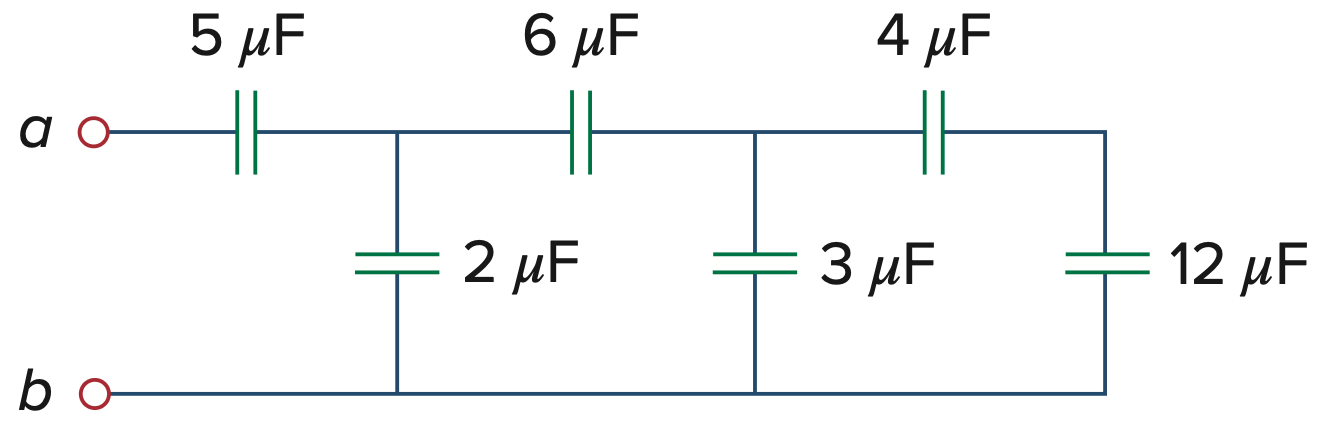
\includegraphics[width=0.7\textwidth]{figures/capacitors_circuit.png}
\end{exercise}

\ifshowsolutions
\begin{solution}
\[
C_{12, 4, 3} = \frac{12\,\mu\mathrm{F} \cdot 4\,\mu\mathrm{F}}{12\,\mu\mathrm{F} + 4\,\mu\mathrm{F}} + 3\,\mu\mathrm{F} = 6\,\mu\mathrm{F}
\]
\[
C_{12, 4, 3, 6, 2} = \frac{C_{4, 12, 3} \cdot 6\,\mu\mathrm{F}}{C_{4, 12, 3} + 6\,\mu\mathrm{F}} + 2\,\mu\mathrm{F} = 5\,\mu\mathrm{F}
\]
\[
C_{a-b} = \frac{C_{12, 4, 3, 6, 2} \cdot 5\,\mu\mathrm{F}}{C_{12, 4, 3, 6, 2} + 5\,\mu\mathrm{F}} = 2.5\,\mu\mathrm{F}
\]
\end{solution}
\fi

\end{document}